\documentclass[letterpaper,12pt,fleqn]{article}
\usepackage{matharticle}
\pagestyle{empty}
\renewcommand{\o}{\theta}
\begin{document}
\section*{Word Problems}

\subsection*{Units}

There is nothing special about a number --- it is just syntax. Numbers become
meaningful when they are used to measure something, and the type of thing that
is being measured is indicated by the units attached to a number.

There are three primitive unit types:
\begin{enumerate}
\item length ($L$)
\item mass (not weight!) ($M$)
\item time ($T$)
\end{enumerate}

All other units are combinations of these three primitive types:
\begin{itemize}
\item Area is $L^2$ - square mile, square meter, acre
\item Volume is $L^3$ - cubic inch, gallon, liter
\item Speed/velocity is $L/T=LT^{-1}$ - mph, miles/hour, meters/second
\end{itemize}

There are three systems of units:
\begin{enumerate}
\item English
\item Meter-Kilogram-Second (mks)
\item Centimeter-Gram-Second (cgs)
\end{enumerate}

In general, problems are solved within a single unit system. This is especially
important when working with derived units:

Weight:

English: $slug$-$ft$/$s^2$=lb (pound) \\
mks: $kg$-$m$/$s^2$=N (newton) \\
cgs: $g$-$cm$/$s^2$=dyn (dyne)

To convert between units of the same type, use a conversion factor:
\[(6 ft)\left(\frac{12 in}{1 ft}\right)=72 in\]
\[(6 ft)\left(\frac{1 yard}{3 ft}\right)=2 yards\]
\[(10 in)\left(\frac{2.54 cm}{1 in}\right)=25.4 cm\]

In equations:
\begin{enumerate}
\item Adding like units
  \[4ft+3in=4ft+3in\left(\frac{1ft}{12in}\right)=4ft+0.25ft=4.25ft\]

\item Combining a rate by an amount to get a total amount
  \[(3ft/s)(10s)=30ft\]

\item Combining values with different units to get a different type of unit
  \[(5 slugs)(32 ft/s^2)=160 lbs\]
\end{enumerate}

These are the three ways that mathematics is used to describe reality. Take the
example of an electomagnet. We have a current (moving electrons) flowing
through a wire (mass) that results in a magnetic field.

\subsection*{Significant Figures}

Don't go crazy with calculator digits. In general, only use as many digits as
are presented in the original problem:

3.1 meter \\
1.6 seconds \\
1.9375 m/s

But each input value was only measured to one decimal place, so the 375 digits
are worthless.

In general, you will be asked to provide an answer to a certain number of
decimal points.

\subsection*{Problem Types}

\begin{enumerate}
\item Percentages (Interest)
\item Distance
\item Mixture
\item Shared Work
\item Triangles
\item Circumference, Area, Volume
\item Falling Object
\end{enumerate}

\begin{example}
  A community theatre group is staging a play in a 100 seat theatre. Adult
  tickets are \$25 and child tickets (12 and under) are \$8. Receipts from
  opening night to a full house are \$2126. How many tickets of each type were
  sold?

  \begin{enumerate}
  \item Be clear on what the answer should look like.

    $n$ adult tickets \\
    $m$ child tickets

  \item Determine what is important and what can be ignored
    \begin{itemize}
    \item 100 seat theatre
    \item ticket prices
    \item full house
    \item Total receipts
    \end{itemize}

  \item Select a key unknown element of the problem and let it be represented
    by a variable:

    Let $x$ be the number of adult tickets sold

  \item Describe other unknown elements in terms of the key element:

    $100-x$ is the number of child tickets sold

  \item Build an equation relating the unknown elements to any restrictions
    using the three types of unit combinations:

    $25x+8(100-x)=2126$

  \item Double-check the units

    adults x \$/adult + kids x \$/kid = \$

  \item Solve for the key unknown:
    \[25x+800-8x=2126\]
    \[17x=1326\]
    \[x=78 adults\]

  \item Determine other unknowns in terms of the key unknown:
    \[kids=100-78=22\]

  \item Clearly state the answer:

    78 adult tickets were sold \\
    22 child tickets were sold
  \end{enumerate}
\end{example}

\subsubsection*{Percentages}

A percentage is a fraction of a whole, expressed as parts per 100:

$3\%$ of 10 is $\left(\frac{3}{100}\right)10=0.03\cdot10=0.3$

Percentage problems usually include and increase or decrease from an original
value:
\[r=\frac{n-o}{o}\]
\[ro=n-o\]
\[n=ro+o\]
\[n=o(1+r)\]
\[p=100*r\]

You have an off-campus job that pays \$180 per week. But you are such a good
worker that your boss gives you a raise and your next paycheck is \$192. What
is the percentage of your raise?
\[180(1+r)=192\]
\[1+r=\frac{192}{180}\]
\[r=\frac{192}{180}-1\]
\[r=0.0\bar{6}=6.\bar{6}\%\]
About a $7\%$ raise

\bigskip

You want to buy a pair of basketball shoes that normally go for \$125, but you
wait until there is a 25\% sale. The sales associate rings you up and says that
the shoes cost \$100. Is this correct?
\[125(1-r)=100\]
\[1-r=\frac{100}{125}\]
\[r=1-\frac{100}{125}\]
\[r=0.20=20\%\]

\subsubsection*{Distance}

rate = distance / time
distance = rate x time
time = distance / rate

Two travelers start from cities 100 km apart. One drives 80 km/h and the other
drives 60 km/h. When and where do they pass each other?
\[60t+80t=100\]
\[140t=100\]
\[t=\frac{100}{140}\cdot60=43 min\]
\[80\cdot\frac{100}{140}=57 km\]

This time, one is traveling 10 mph faster than the other. In the same amount of
time, the first goes 140 miles but the second only 120 miles.  How fast is
each driver going?
\[\frac{120}{r}=\frac{140}{r+10}\]
\[120(r+10)=140r\]
\[120r+1200=140r\]
\[20r=1200\]
\[r=60 mph\]
Driver 1: 70 mph \\
Driver 2: 60 mph

\subsubsection*{Mixtures}

The ticket and the first driving problem are all examples of \emph{mixture}
problems:
\[r_1a_1+r_2a_2=r_3(a_1+a_2)\]

$r=\frac{miles}{hour}$, $a=hours$ \\
$r=\frac{kg}{L}$, $a=L$ \\

Peanuts cost \$5 per pound and cashews cost \$7.50 per pound
Mix 10 lb of peanuts and 5 lb of cashews
What should the price per pound be for the mixture?

$r_1=5 \$/lb$, $a_1=10 lb$ \\
$r_2=7.50 \$/lb$, $a_2=5 lb$ \\
$x=$ price per pound of mixture \\
\[5(10)+7.5(5)=(10+5)x\]
\[50+37.50=15x\]
\[15x=87.50\]
\[x=5.84\]
The mixture should be sold at \$5.84 per pound.

\subsubsection*{Shared Work}

\[r_1+r_2=r_3\]

A hose from one spigot can fill a small pool in 40 min. A hose from a
different spigot can fill the same pool in 65 min. How long does it take to
fill the pool if both sources of water are used?

The rates here are jobs per minutes, where the number of jobs is typically 1.

\[\frac{1}{40}+\frac{1}{65}=\frac{1}{x}\]
\[\frac{65+40}{40(65)}=\frac{1}{x}\]
\[\frac{105}{2600}=\frac{1}{x}\]
\[105x=2600\]
\[x=24.8\]

About 25 minutes

\subsubsection*{Triangles}

Similar triangles:

\begin{minipage}[t]{3in}
  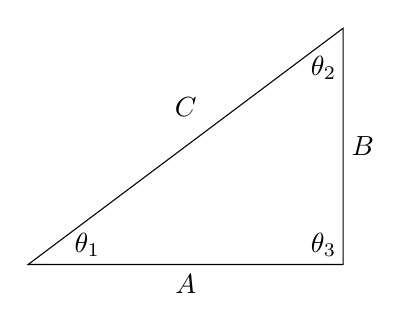
\begin{tikzpicture}
    \draw (0,0) -- (4,0) -- (4,3) -- cycle;
    \node at (0.75,0.25) {$\o_1$};
    \node at (3.75,2.5) {$\o_2$};
    \node at (3.75,0.25) {$\o_3$};
    \node at (2,2) {$C$};
    \node at (4.25,1.5) {$B$};
    \node at (2,-0.25) {$A$};
  \end{tikzpicture}
\end{minipage}
\begin{minipage}[t]{3in}
  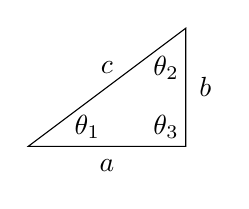
\begin{tikzpicture}
    \draw (0,0) -- (2,0) -- (2,1.5) -- cycle;
    \node at (0.75,0.25) {$\o_1$};
    \node at (1.75,1) {$\o_2$};
    \node at (1.75,0.25) {$\o_3$};
    \node at (1,1) {$c$};
    \node at (2.25,0.75) {$b$};
    \node at (1,-0.25) {$a$};
  \end{tikzpicture}
\end{minipage}
\newpage
Ratios match:
\[\frac{a}{A}=\frac{b}{B}=\frac{c}{C}\]
Can also mix:
\[aB=Ab\]
\[\frac{a}{b}=\frac{A}{B}\]

A building casts a 25 foot shadow. You place a 5 foot pole at the end of the
shadow. The pole casts a 2 foot shadow. How tall is the building?

\begin{minipage}[t]{3in}
  \begin{tikzpicture}
    \draw (-3,-2) -- (3,2);
    \draw (-3,2) -- (3,-2);
    \node at (-0.5,0) {$\o$};
    \node at (0.5,0) {$\o$};
  \end{tikzpicture}
\end{minipage}
\begin{minipage}[t]{3in}
  \begin{tikzpicture}
    \draw (-3,2) -- (3,-2);
    \draw (-3,1) -- (3,1);
    \draw (-3,-1) -- (3,-1);
    \node at (-2.25,1.25) {$\o$};
    \node at (-0.75,0.75) {$\o$};
    \node at (2.25,-1.25) {$\o$};
    \node at (0.75,-0.75) {$\o$};
  \end{tikzpicture}
\end{minipage}

The sun is so far away that all of its rays hitting the earth can be assumed
to be parallel. So, the building/shadow and pole/shadow make similar triangles:
\[\frac{x}{25}=\frac{5}{2}\]
\[2x=125\]
\[x=62.5\]
The building is 62.5 feet tall.

\bigskip

Right Triangles:

Pythagorean Theorem

\begin{minipage}{3in}
  \begin{tikzpicture}
    \draw (0,0) -- (0,3) -- (4,0) -- cycle;
    \node at (2,2) {$c$};
    \node at (2,-0.25) {$b$};
    \node at (-0.25,1.5) {$a$};
  \end{tikzpicture}
\end{minipage}
\begin{minipage}{3in}
  $a^2+b^2=c^2$

  $3,4,5$ \\
  $5,12,13$ \\
  $6,8,10$ \\
  $8,15,17$ \\
  $7,24,25$
\end{minipage}

You wish to measure how high up a window is in the side of a building. You
have a 13 foot ladder and a measuring tape. By placing the top of the ladder
at the bottom of the window, the bottom of the ladder is 5 feet away from the
bottom of the building. How high is the window?

\[5^2+h^2=13^2\]
\[25+h^2=169\]
\[h^2=144\]
\[h=12\]
The window is 12 feet up the side of the building.

\subsubsection*{Circumference, Area, Volume}

See page 86 for some common formulas.

A farmer has 1200ft of fencing. He wants to build a horse enclosure that is
twice as long as it is wide. What are the dimensions of the enclosure?

\bigskip

\begin{tikzpicture}
  \draw (0,0) rectangle (4,3);
  \node [below] at (2,0) {$\ell$};
  \node [right] at (4,1.5) {$w$};
  \node at (8,1.5) {$C=2\ell+2w$};
\end{tikzpicture}

$w=x$ \\
$\ell=2x$ \\
$2x+2(2x)=1200$ \\
$6x=1200$ \\
$x=200$

$w=200$ \\
$\ell=400$

The enclosure should be 400 feet by 200 feet.

\bigskip

A car tire has a radius of 16 inches. Tires are to be replaced after 50,000
miles. How many rotations before replacement?

\bigskip

\begin{tikzpicture}
  \draw (0,0) circle [radius=2];
  \draw [dashed] (0,0) -- (2,0);
  \node [above] at (1,0) {$r$};
  \node at (6,0) {$C=2\pi r$};
\end{tikzpicture}

$n =$ number of rotations

$(2\pi r$ in/rev$)(n$ revs$)=(50000$ mi$)(5280$ ft/mi$)(12$ in/ft)

$n=\frac{50000(5280)(10)}{2\pi(16)}=31.5$ million

\bigskip

A rectangular garden is 30 feet long and 20 feet wide. It is surrounded on all
sides by a rock path of equal width. The total area of the garden and path is
1200 square feet. How wide is the path?

\bigskip

\begin{tikzpicture}
  \draw (0,0) rectangle (4,3);
  \draw (0.5,0.5) rectangle (3.5,2.5);
  \node [above] at (2,0.5) {$30$};
  \node [right] at (0.5,1.5) {$20$};
  \node at (3.8,1.5) {$x$};
  \node at (8,1.5) {$A=w\ell=1200$ sq ft};
\end{tikzpicture}

$x=$ width of path
\[(2x+20)(2x+30)=1200\]
\[4(x+10)(x+15)=1200\]
\[(x+10)(x+15)=300\]
\[x^2+25x+150=300\]
\[x^2+25x-150=0\]
\[(x+30)(x-5)=0\]
\[x=-30,5\]
The path is 5 feet wide.

\subsubsection*{Falling Object}

Set up a coordinate system, establishing a reference point (0) and the
direction of positive motion.

s=displacement \\
v=velocity=change in displacement per unit time \\
a=acceleration=change in speed per unit time

Motion under constant acceleration:
\[s=s_0+v_0t+\frac{1}{2}at^2\]

Gravity, near the surface of the earth, results in constant acceleration:
objects moving with gravity go continually faster and objects moving against
gravity move continually slower.

\[g=32 ft/s^2\]
\[g=9.8 m/s^2\]

A man stands on a 256 foot cliff with a red ball:
\begin{enumerate}
\item simply drops the ball
\item throws the ball up with an initial velocity of 5 ft/s
\item throws the ball down with an initial velocity of 5 ft/s
\end{enumerate}

\[s=256+v_0t+\frac{1}{2}(-32)t^2)\]
\[s=256+v_0t-16t^2)\]

Case 1: $v_0=0$
\[0=256-16t^2\]
\[16t^2=256\]
\[t^2=16\]
\[t=\pm4\]

Case 2: $v_0=5$ ft/s
\[0=256+5t-16t^2\]
\[16t^2-5t-256=0\]
\[t=\frac{5\pm\sqrt{5^2-4(16)(-256)}}{2(16)}\]
\[t=-3.85,4.16\]

Case 3: $v_0=-5$ ft/s
\[0=256-5t-16t^2\]
\[16t^2+5t-256=0\]
\[t=\frac{-5\pm\sqrt{(-5)^2-4(16)(-256)}}{2(16)}\]
\[t=-4.16,3.85\]
\end{document}
